\begin{name}
	{\tenchude}
	{\tendethi}
	{\tentruong}
	{\thoigian}
\end{name} 
\Opensolutionfile{ans}[ans/ansKTCT12]

\TN \textit{(3,0 điểm)}

\begin{ex}%[BG 11 - Nguyen Huynh]%[1D1V4-3][Mức độ 3]
Trong các hàm số sau, hàm số nào đồng biến trên khoảng $\left(-\dfrac{\pi}{3};\dfrac{\pi}{6}\right)$?
\choice
{$y=\cot \left(2x+\dfrac{\pi}{6}\right)$}
{$y=\cos \left(2x+\dfrac{\pi}{6}\right)$}
{\True $y=\sin \left(2x+\dfrac{\pi}{6}\right)$}
{$y=\tan \left(2x+\dfrac{\pi}{6}\right)$}
\loigiai{
Với $x\in \left(-\dfrac{\pi}{3};\dfrac{\pi}{6}\right)\Rightarrow 2x\in \left(-\dfrac{2\pi}{3};\dfrac{\pi}{3}\right)\Rightarrow 2x+\dfrac{\pi}{6}\in \left(-\dfrac{\pi}{2};\dfrac{\pi}{2}\right)$ thuộc góc phần tư thứ IV và thứ nhất nên hàm số $y=\sin \left(2x+\dfrac{\pi}{6}\right)$ đồng biến trên khoảng $\left(-\dfrac{\pi}{3};\dfrac{\pi}{6}\right)$.}
\end{ex}

\begin{ex}%[VN-MT-9]%[1-TK-HK1-KN-5-2425, Khổng Xuân Thạnh]%[1D1N1-5]
    \immini[thm]{
Cho góc $\alpha$ được biểu diễn trên đường tròn lượng giác như hình vẽ. Mệnh đề nào dưới đây đúng?
\choice
{$\sin \alpha \cdot \cos \alpha >0$}
{\True $\sin \alpha -\dfrac{1}{2}>0$}
{$\tan \alpha \cdot \cot \alpha <0$}
{$\sin \alpha <0<\cos \alpha$}
    }{\begin{tikzpicture}[scale=0.5, font=\footnotesize, line join=round, line cap=round, >=stealth]
\path (0,0) coordinate (O)
(3,0) coordinate (A)
(0,3) coordinate (B)
(0,-3) coordinate (B')
(-3,0) coordinate (A')
(120:3) coordinate (M);
\draw[->] (-4,0) -- (4,0) node[above]{$x$};
\draw[->] (0,-4) -- (0,4) node[left]{$y$};
\draw (O) circle (3cm);
\draw[rotate=0,->] (0.5,0) arc (0:120:0.5cm); % Điều chỉnh góc quay cho M
\draw (M)--(O);
\foreach \p/\r in {M/75}
\fill (\p) circle (1pt) node[shift={(\r+50:3mm)},]{$\p$};
\fill (O) circle (1pt) node[below left] {$O$};
\draw pic[draw=none,"$\alpha$",angle radius=10mm]{angle=A--O--M};
\end{tikzpicture}}
\loigiai{
Góc $\alpha$ được biểu diễn như hình vẽ, khi đó $\sin \alpha>0$, $\cos \alpha<0$, $\tan \alpha<0$, $\cot \alpha <0$.
\begin{center}
\begin{tikzpicture}[scale=0.6, font=\footnotesize, line join=round, line cap=round, >=stealth]
\path (0,0) coordinate (O)
(3,0) coordinate (A)
(0,3) coordinate (B)
(0,1.5) coordinate (C)
(0,-3) coordinate (B')
(-3,0) coordinate (A')
(120:3) coordinate (M)
(90:2.65) coordinate (N);
\draw[->] (-4,0) -- (4,0) node[above]{$x$};
\draw[->] (0,-4) -- (0.,4) node[left]{$y$};
\draw (O) circle (3cm);
\draw[rotate=0,->] (0.5,0) arc (0:120:0.5cm); % Điều chỉnh góc quay cho M
\draw (M)--(O);
\draw[dashed,] (M)--(N);
\foreach \p/\r in {M/75}
\fill (\p) circle (1pt) node[shift={(\r+50:3mm)},]{$\p$};
\fill (O) circle (1pt) node[below left] {$O$};
\fill (C) circle (2pt) node[left] {$\frac{1}{2}$};
\draw pic[draw=none,"$\alpha$",angle radius=10mm]{angle=A--O--M};
\end{tikzpicture}
\end{center}
Tung độ của điểm $M$ là $\sin \alpha$ suy ra $\sin \alpha >\dfrac{1}{2}$.\\
Mệnh đề đúng là $\sin \alpha -\dfrac{1}{2}>0$.
}
\end{ex}

\begin{ex}%[1D1N2-4]%[KNTT - Lớp 11 - Ôn tập cuối học kì 1 - Đề 3]%[Võ Thị Thùy Trang]
Cho hai góc $\alpha$, $\beta$ thỏa mãn $\alpha+\beta=\dfrac{\pi}{2}$. Hỏi khẳng định nào sau đây đúng?
\choice
{$\sin \alpha=\sin \beta$}
{\True $\sin \alpha=\cos \beta$}
{$\sin \alpha=-\cos \beta$}
{$\sin \alpha=-\sin \beta$}
\loigiai{
Vì $\alpha+\beta=\dfrac{\pi}{2}$ nên $\sin \alpha=\sin \left(\dfrac{\pi}{2}-\beta\right)=\cos \beta$.
}
\end{ex}

\begin{ex}%[Đề thi HK1 trường THTH ĐHSP TP.HCM năm 2023-2024]%[Nguyễn Tấn Linh, dự án 10-11-EX-HK1-2324]%[1D1N3-4]
Mệnh đề nào sau đây \textbf{sai}?
\choice
{\True $\sin a\cos b=\dfrac{1}{2}\left[\sin (a-b)-\cos (a+b)\right]$}
{$\sin a\sin b=\dfrac{1}{2}\left[\cos (a-b)-\cos (a+b)\right]$}
{$\sin a\cos b=\dfrac{1}{2}\left[\sin (a-b)+\sin (a+b)\right]$}
{$\cos a\cos b=\dfrac{1}{2}\left[\cos (a-b)+\cos (a+b)\right]$}
\loigiai
{$\sin a\cos b=\dfrac{1}{2}\left[\sin (a-b)+\sin (a+b)\right]$.
}
\end{ex}

\begin{ex}%[Đề thi HK 1 Lớp 11- THPT Núi Thành - Quảng Nam, Năm học 2023-2024]%[Tran Quoc, 10-11-HK1-2024]%[1D1N4-2]
Hàm số $y=\tan x$ không xác định tại điểm nào dưới đây?
\choice
{$x=0$}
{\True $x=\dfrac{3 \pi}{2}$}
{$x=\dfrac{3 \pi}{4}$}
{$x=\dfrac{\pi}{4}$}
\loigiai{Hàm số $y=\tan x$ xác định khi và chỉ khi $\cos x \ne 0 \Leftrightarrow x \ne \dfrac{\pi}{2}+k \pi$, $k \in \mathbb{Z}$.\\
Do đó, hàm số $y=\tan x$ gián đoạn tại $x=\dfrac{3\pi}{2}$.}
\end{ex}

\begin{ex}%[1-HK1-KN-6-DoanKet-HaNoi-2324]%[VN-MT-6,VM017] %[1D1N5-1]
Phương trình $\sin x=\sin \beta$ có nghiệm là
\choice
{$\hoac{&x=\beta+k \pi \\
&x=-\beta+k \pi}; k \in \mathbb{Z}$}
{$\hoac{&x=\beta+k 2\pi \\
&x=-\beta+k 2\pi}; k \in \mathbb{Z}$}
{$\hoac{&x=\beta+k \pi \\
&x=\pi-\beta+k \pi}; k \in \mathbb{Z}$}
{\True $\hoac{&x=\beta+k 2\pi \\
&x=\pi-\beta+k 2\pi}; k \in \mathbb{Z}$}
\loigiai{
Ta có $\sin x=\sin \beta \Leftrightarrow \hoac{&x=\beta+k 2\pi \\
&x=\pi-\beta+k 2\pi}; k \in \mathbb{Z}$
}
\end{ex}

\TNTF \textit{(4,0 điểm)}
\begin{ex}%[Hoàng Thanh Phương, 24-25 BG K11]%[1D1H3-3]
Cho $\sin\alpha=\dfrac{3}{5}$ và $\cos \alpha=-\dfrac{4}{5}$. Mỗi khẳng định dưới đây đúng hay sai?
\choiceTF
{$\sin2\alpha=\dfrac{6}{5}$}
{\True $\cos2\alpha=\dfrac{7}{25}$}
{\True $\tan2\alpha=-\dfrac{24}{7}$}
{\True $\cot2\alpha=-\dfrac{7}{24}$}
\loigiai{
\begin{itemchoice}
\itemch $\sin2\alpha=2\sin\alpha\cos\alpha=2\cdot\dfrac{3}{5}\cdot\left(-\dfrac{4}{5}\right)=-\dfrac{24}{25}$.
\itemch $\cos2\alpha=1-2\sin^2\alpha=1-2\left(\dfrac{3}{5}\right)^2=\dfrac{7}{25}$.
\itemch $\tan2\alpha=\dfrac{\sin2\alpha}{\cos2\alpha}=-\dfrac{24}{25}:\dfrac{7}{25}=-\dfrac{24}{7}.$
\itemch $\cot2\alpha=\dfrac{1}{\tan2\alpha}=-\dfrac{7}{24}.$
\end{itemchoice}
}
\end{ex}

\begin{ex}%[De-chuan-hoa-so-25]%[Phạm Ngọc Trung]%[1D1H5-3]
Cho hai đồ thị hàm số $y=f(x)=\sin\left(x+\dfrac{\pi}{4}\right)$ và $y=g(x)=\sin x$, khi đó
\choiceTF[t]
{\True Hàm số $f\left(x\right)$ có chu kì là $2\pi$}
{\True Hoành độ giao điểm của hai đồ thị là $x=\dfrac{3\pi}{8}+k\pi$, $k\in\mathbb{Z}$}
{Khi $x\in[0;2\pi]$ thì hai đồ thị hàm số cắt nhau tại ba điểm}
{Gọi $T$ (rad) là nghiệm dương nhỏ nhất của phương trình $f(x)$. Cho biết kim giờ và kim phút của một đồng hồ lớn có độ dài lần lượt là $17{,}5$ cm và $23{,}5$ cm. Khi kim phút quay được một góc có số đo bằng $T$ (rad) thì kim giờ và kim phút vạch được các cung tròn có tổng độ dài lớn hơn $49$\,cm}
\loigiai{Phương trình hoành độ giao điểm của hai đồ thị hàm số là
\[\sin\left(x+\dfrac{\pi}{4}\right)=\sin x\Leftrightarrow\hoac{&x+\dfrac{\pi}{4}=x+k2\pi\\&x+\dfrac{\pi}{4}=\pi-x+k2\pi}\Leftrightarrow x=\dfrac{3\pi}{8}+k\pi\quad(k\in\mathbb{Z}).\]
Vì $x\in[0;2\pi]$ nên $x\in\left\{\dfrac{3\pi}{8};\dfrac{11\pi}{8}\right\}$.\\
Với $x=\dfrac{3\pi}{8}\Rightarrow y=\sin\dfrac{3\pi}{8}$, với $x=\dfrac{11\pi}{8}\Rightarrow y=\sin\dfrac{11\pi}{8}$.\\
Vậy toạ độ giao điểm của hai đồ thị hàm số là $\left(\dfrac{3\pi}{8};\sin\dfrac{3\pi}{8}\right),\left(\dfrac{11\pi}{8};\sin\dfrac{11\pi}{8}\right)$.
\begin{itemchoice}
\itemch Phương trình hoành độ giao điểm của hai đồ thị hàm số là $\sin\left(x+\dfrac{\pi}{4}\right)=\sin x$ là đúng.
\itemch Hoành độ giao điểm của hai đồ thị là $x=\dfrac{3\pi}{8}+k\pi$, $k\in\mathbb{Z}$ là đúng.
\itemch Khi $x\in[0;2\pi]$ thì hai đồ thị hàm số cắt nhau tại ba điểm là sai.
\itemch Phương trình $f(x)=g(x)$ có nghiệm dương nhỏ nhất bằng $\dfrac{3\pi}{8}$.\\
Theo đề bài ta có kim phút quay được một góc có số đo là $\dfrac{3\pi}{8}$ (rad).\\
Khi đó kim giờ quay được góc có số đo là \[\dfrac{1}{12}\cdot \dfrac{3\pi}{8}=\dfrac{\pi}{32}.\]
Suy ra tổng độ dài các cung tròn mà kim phút và kim giờ quay được là
\[\ell=\dfrac{3\pi}{8} \cdot 23{,}5+\dfrac {\pi}{32}\cdot 17{,}5\approx 29{,}4\,\text{(cm)}.\]
\end{itemchoice}}
\end{ex}

\TNSA \textit{(2,0 điểm)}

\begin{ex}%[Cánh diều]%[Đỗ Vũ Minh Thắng, 24-25 BG 10 11]%[1D1V3-2]
\immini[thm]{Có hai chung cư cao tầng xây cạnh nhau với khoảng cách giữa chúng là $H K=20 \mathrm{~m}$. Để đảm bảo an ninh, trên nóc chung cư thứ hai người ta lắp camera ở vị trí $C$. Gọi $A, B$ lần lượt là vị trí thấp nhất, cao nhất trên chung cư thứ nhất mà camera có thể quan sát được (Hình dưới). Hãy tính số đo góc $A C B$ (phạm vi camera có thể quan sát được ở chung cư thứ nhất). Biết rằng chiều cao của chung cư thứ hai là $C K=32 \mathrm{~m}$, $A H=6 \mathrm{~m}, B H=24 \mathrm{~m}$ (làm tròn kết quả đến hàng phần mười theo đơn vị độ).
\shortans{30,6}
}{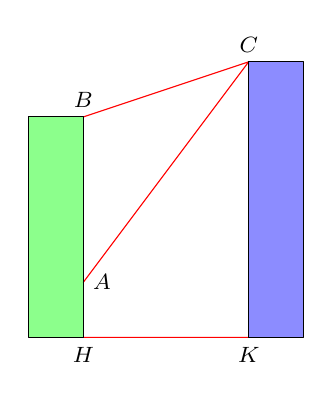
\begin{tikzpicture}[>=stealth,line join=round,line cap=round,font=\footnotesize,scale=.7]
\path
(0,0) coordinate (H)node[below]{$H$}
(-1,0) coordinate (H1)
(0,1) coordinate (A)node[right]{$A$}
(0,4) coordinate (B)node[above]{$B$}
(-1,4) coordinate (B1)
(3,0) coordinate (K)node[below]{$K$}
(4,0) coordinate (K1)
(3,5) coordinate (C)node[above]{$C$}
(4,5) coordinate (C1)
;
\fill[green!45]
(H)--(B)--(B1)--(H1)--cycle
;
\fill[blue!45]
(C)--(K)--(K1)--(C1)--cycle
;
\draw[red]
(B)--(C)
(A)--(C)
(H)--(K)
;
\draw[black]
(H)--(B)--(B1)--(H1)--cycle
(C)--(K)--(K1)--(C1)--cycle
;
\end{tikzpicture}}
\loigiai{
\immini{Ta có $CD=CK-BH=8$, $CI=CK-AH=26$, $BD=AI=HK=20$.\\
$\tan\widehat{BCD}=\dfrac{BD}{CD}=\dfrac{20}{8}=\dfrac{5}{2}$, $\tan\widehat{ACI}=\dfrac{AI}{CI}=\dfrac{20}{26}=\dfrac{10}{13}$.\\
$\tan\widehat{BCA}=\tan\left(\widehat{BCD}-\widehat{ACI}\right)=\dfrac{\tan\widehat{BCD}-\tan\widehat{ACI}}{1+\tan\widehat{BCD}.\tan\widehat{ACI}}=\dfrac{\frac{5}{2}-\frac{10}{13}}{1+\frac{5}{2}\cdot\frac{10}{13}}$\\
$\tan\widehat{BCA}=\dfrac{45}{76}\Rightarrow \widehat{BCA}\approx 30,6^\circ $.

}
{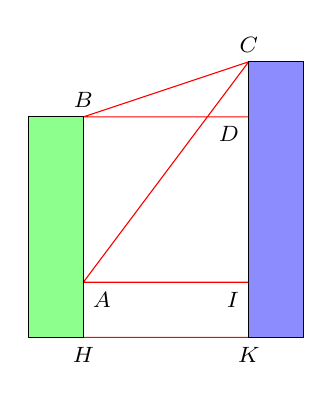
\begin{tikzpicture}[>=stealth,line join=round,line cap=round,font=\footnotesize,scale=.7]
\path
(0,0) coordinate (H)node[below]{$H$}
(-1,0) coordinate (H1)
(0,1) coordinate (A)node[below right]{$A$}
(0,4) coordinate (B)node[above]{$B$}
(-1,4) coordinate (B1)
(3,0) coordinate (K)node[below]{$K$}
(4,0) coordinate (K1)
(3,5) coordinate (C)node[above]{$C$}
(4,5) coordinate (C1)
(3,4) coordinate (D)node[below left]{$D$}
(3,1) coordinate (I)node[below left]{$I$}
;
\fill[green!45]
(H)--(B)--(B1)--(H1)--cycle
;
\fill[blue!45]
(C)--(K)--(K1)--(C1)--cycle
;
\draw[red]
(B)--(C)
(A)--(C)
(H)--(K)
(B)--(D)
(A)--(I)
;
\draw[black]
(H)--(B)--(B1)--(H1)--cycle
(C)--(K)--(K1)--(C1)--cycle
;
\end{tikzpicture}
}
}
\end{ex}

\begin{ex}%[1D1V5-5]
Tổng tất cả các nghiệm trên đoạn $[-\pi;\pi]$ của phương trình $\cos 2x+\sqrt{3}\sin 2x=\sqrt{2}$ là $\dfrac{-a\pi}{b}$ với $\dfrac{a}{b}$ là phân số tối giản. Giá trị của $a+b$ là
\shortans[]{$7$}
\loigiai{	{\allowdisplaybreaks
\begin{eqnarray*}
& &\cos 2x+\sqrt{3}\sin 2x=\sqrt{2}
\Leftrightarrow
\dfrac{\sqrt{3}}{2}\sin 2x+\dfrac{1}{2}\cos2x=\dfrac{\sqrt{2}}{2}\\
&\Leftrightarrow&
\sin\left(2x+\dfrac{\pi}{6}\right)=\sin\dfrac{\pi}{4}
\Leftrightarrow
\hoac{&x=\dfrac{\pi}{24}+k\pi\\&x=\dfrac{7\pi}{24}+k\pi}, (k\in\mathbb{Z}).
\end{eqnarray*}
}
Trên đoạn $[-\pi;\pi]$ họ $x=\dfrac{\pi}{24}+k\pi$ có hai   nghiệm là $\dfrac{\pi}{24}$ và $\dfrac{\pi}{24}-\pi$.\\
Trên đoạn $[-\pi;\pi]$ họ $x=\dfrac{7\pi}{24}+k\pi$ có hai nghiệm là $\dfrac{7\pi}{24}$ và $\dfrac{7\pi}{24}-\pi$.\\
Do đó tổng tất cả các nghiệm là $-\dfrac{4\pi}{3}$.\\
Vậy $a=4$, $b=3$ nên $a+b=7$.
}
\end{ex}
\Closesolutionfile{ans}
\inputansbox{4}{ans/ansKTCT12}
\TL \textit{(2,0 điểm)}
\begin{ex}%[1D1H5-5]
Giải các phương trình sau
\begin{listEX}[2]
\item $2\sin x+\sqrt{2}=0$;
\item $\sin2x-2\sin x=0$.
\end{listEX}
\loigiai{
\begin{enumerate}[a)]
\item $2\sin x+\sqrt{2}=0\Leftrightarrow\sin x=-\dfrac{\sqrt{2}}{2}\Leftrightarrow\sin x=\sin\left(-\dfrac{\pi}{4}\right)\Leftrightarrow\hoac{&x=-\dfrac{\pi}{4}+k2\pi\\&x=\dfrac{5\pi}{4}+k2\pi}\,(k\in\mathbb{Z})$;
\item $\sin 2x - 2\sin x=0 \Leftrightarrow 2\sin x \cos x - 2\sin x=0 \Leftrightarrow 2\sin x (\cos x -1)=0 \Leftrightarrow \hoac{& \sin x =0 \\ & \cos x =1} \Leftrightarrow \sin x =0 \Leftrightarrow x = k\pi (k \in \mathbb{Z})$
\end{enumerate}
}
\end{ex}
\dongcham{10}
